% Options for packages loaded elsewhere
\PassOptionsToPackage{unicode}{hyperref}
\PassOptionsToPackage{hyphens}{url}
\PassOptionsToPackage{dvipsnames,svgnames,x11names}{xcolor}
%
\documentclass[
  letterpaper,
  DIV=11,
  numbers=noendperiod,
  oneside]{scrartcl}

\usepackage{amsmath,amssymb}
\usepackage{lmodern}
\usepackage{iftex}
\ifPDFTeX
  \usepackage[T1]{fontenc}
  \usepackage[utf8]{inputenc}
  \usepackage{textcomp} % provide euro and other symbols
\else % if luatex or xetex
  \usepackage{unicode-math}
  \defaultfontfeatures{Scale=MatchLowercase}
  \defaultfontfeatures[\rmfamily]{Ligatures=TeX,Scale=1}
\fi
% Use upquote if available, for straight quotes in verbatim environments
\IfFileExists{upquote.sty}{\usepackage{upquote}}{}
\IfFileExists{microtype.sty}{% use microtype if available
  \usepackage[]{microtype}
  \UseMicrotypeSet[protrusion]{basicmath} % disable protrusion for tt fonts
}{}
\makeatletter
\@ifundefined{KOMAClassName}{% if non-KOMA class
  \IfFileExists{parskip.sty}{%
    \usepackage{parskip}
  }{% else
    \setlength{\parindent}{0pt}
    \setlength{\parskip}{6pt plus 2pt minus 1pt}}
}{% if KOMA class
  \KOMAoptions{parskip=half}}
\makeatother
\usepackage{xcolor}
\usepackage[left=1in,marginparwidth=2.0666666666667in,textwidth=4.1333333333333in,marginparsep=0.3in]{geometry}
\setlength{\emergencystretch}{3em} % prevent overfull lines
\setcounter{secnumdepth}{5}
% Make \paragraph and \subparagraph free-standing
\ifx\paragraph\undefined\else
  \let\oldparagraph\paragraph
  \renewcommand{\paragraph}[1]{\oldparagraph{#1}\mbox{}}
\fi
\ifx\subparagraph\undefined\else
  \let\oldsubparagraph\subparagraph
  \renewcommand{\subparagraph}[1]{\oldsubparagraph{#1}\mbox{}}
\fi

\usepackage{color}
\usepackage{fancyvrb}
\newcommand{\VerbBar}{|}
\newcommand{\VERB}{\Verb[commandchars=\\\{\}]}
\DefineVerbatimEnvironment{Highlighting}{Verbatim}{commandchars=\\\{\}}
% Add ',fontsize=\small' for more characters per line
\usepackage{framed}
\definecolor{shadecolor}{RGB}{241,243,245}
\newenvironment{Shaded}{\begin{snugshade}}{\end{snugshade}}
\newcommand{\AlertTok}[1]{\textcolor[rgb]{0.68,0.00,0.00}{#1}}
\newcommand{\AnnotationTok}[1]{\textcolor[rgb]{0.37,0.37,0.37}{#1}}
\newcommand{\AttributeTok}[1]{\textcolor[rgb]{0.40,0.45,0.13}{#1}}
\newcommand{\BaseNTok}[1]{\textcolor[rgb]{0.68,0.00,0.00}{#1}}
\newcommand{\BuiltInTok}[1]{\textcolor[rgb]{0.00,0.23,0.31}{#1}}
\newcommand{\CharTok}[1]{\textcolor[rgb]{0.13,0.47,0.30}{#1}}
\newcommand{\CommentTok}[1]{\textcolor[rgb]{0.37,0.37,0.37}{#1}}
\newcommand{\CommentVarTok}[1]{\textcolor[rgb]{0.37,0.37,0.37}{\textit{#1}}}
\newcommand{\ConstantTok}[1]{\textcolor[rgb]{0.56,0.35,0.01}{#1}}
\newcommand{\ControlFlowTok}[1]{\textcolor[rgb]{0.00,0.23,0.31}{#1}}
\newcommand{\DataTypeTok}[1]{\textcolor[rgb]{0.68,0.00,0.00}{#1}}
\newcommand{\DecValTok}[1]{\textcolor[rgb]{0.68,0.00,0.00}{#1}}
\newcommand{\DocumentationTok}[1]{\textcolor[rgb]{0.37,0.37,0.37}{\textit{#1}}}
\newcommand{\ErrorTok}[1]{\textcolor[rgb]{0.68,0.00,0.00}{#1}}
\newcommand{\ExtensionTok}[1]{\textcolor[rgb]{0.00,0.23,0.31}{#1}}
\newcommand{\FloatTok}[1]{\textcolor[rgb]{0.68,0.00,0.00}{#1}}
\newcommand{\FunctionTok}[1]{\textcolor[rgb]{0.28,0.35,0.67}{#1}}
\newcommand{\ImportTok}[1]{\textcolor[rgb]{0.00,0.46,0.62}{#1}}
\newcommand{\InformationTok}[1]{\textcolor[rgb]{0.37,0.37,0.37}{#1}}
\newcommand{\KeywordTok}[1]{\textcolor[rgb]{0.00,0.23,0.31}{#1}}
\newcommand{\NormalTok}[1]{\textcolor[rgb]{0.00,0.23,0.31}{#1}}
\newcommand{\OperatorTok}[1]{\textcolor[rgb]{0.37,0.37,0.37}{#1}}
\newcommand{\OtherTok}[1]{\textcolor[rgb]{0.00,0.23,0.31}{#1}}
\newcommand{\PreprocessorTok}[1]{\textcolor[rgb]{0.68,0.00,0.00}{#1}}
\newcommand{\RegionMarkerTok}[1]{\textcolor[rgb]{0.00,0.23,0.31}{#1}}
\newcommand{\SpecialCharTok}[1]{\textcolor[rgb]{0.37,0.37,0.37}{#1}}
\newcommand{\SpecialStringTok}[1]{\textcolor[rgb]{0.13,0.47,0.30}{#1}}
\newcommand{\StringTok}[1]{\textcolor[rgb]{0.13,0.47,0.30}{#1}}
\newcommand{\VariableTok}[1]{\textcolor[rgb]{0.07,0.07,0.07}{#1}}
\newcommand{\VerbatimStringTok}[1]{\textcolor[rgb]{0.13,0.47,0.30}{#1}}
\newcommand{\WarningTok}[1]{\textcolor[rgb]{0.37,0.37,0.37}{\textit{#1}}}

\providecommand{\tightlist}{%
  \setlength{\itemsep}{0pt}\setlength{\parskip}{0pt}}\usepackage{longtable,booktabs,array}
\usepackage{calc} % for calculating minipage widths
% Correct order of tables after \paragraph or \subparagraph
\usepackage{etoolbox}
\makeatletter
\patchcmd\longtable{\par}{\if@noskipsec\mbox{}\fi\par}{}{}
\makeatother
% Allow footnotes in longtable head/foot
\IfFileExists{footnotehyper.sty}{\usepackage{footnotehyper}}{\usepackage{footnote}}
\makesavenoteenv{longtable}
\usepackage{graphicx}
\makeatletter
\def\maxwidth{\ifdim\Gin@nat@width>\linewidth\linewidth\else\Gin@nat@width\fi}
\def\maxheight{\ifdim\Gin@nat@height>\textheight\textheight\else\Gin@nat@height\fi}
\makeatother
% Scale images if necessary, so that they will not overflow the page
% margins by default, and it is still possible to overwrite the defaults
% using explicit options in \includegraphics[width, height, ...]{}
\setkeys{Gin}{width=\maxwidth,height=\maxheight,keepaspectratio}
% Set default figure placement to htbp
\makeatletter
\def\fps@figure{htbp}
\makeatother

\KOMAoption{captions}{tableheading}
\makeatletter
\makeatother
\makeatletter
\makeatother
\makeatletter
\@ifpackageloaded{caption}{}{\usepackage{caption}}
\AtBeginDocument{%
\ifdefined\contentsname
  \renewcommand*\contentsname{Table of contents}
\else
  \newcommand\contentsname{Table of contents}
\fi
\ifdefined\listfigurename
  \renewcommand*\listfigurename{List of Figures}
\else
  \newcommand\listfigurename{List of Figures}
\fi
\ifdefined\listtablename
  \renewcommand*\listtablename{List of Tables}
\else
  \newcommand\listtablename{List of Tables}
\fi
\ifdefined\figurename
  \renewcommand*\figurename{Figure}
\else
  \newcommand\figurename{Figure}
\fi
\ifdefined\tablename
  \renewcommand*\tablename{Table}
\else
  \newcommand\tablename{Table}
\fi
}
\@ifpackageloaded{float}{}{\usepackage{float}}
\floatstyle{ruled}
\@ifundefined{c@chapter}{\newfloat{codelisting}{h}{lop}}{\newfloat{codelisting}{h}{lop}[chapter]}
\floatname{codelisting}{Listing}
\newcommand*\listoflistings{\listof{codelisting}{List of Listings}}
\makeatother
\makeatletter
\@ifpackageloaded{caption}{}{\usepackage{caption}}
\@ifpackageloaded{subcaption}{}{\usepackage{subcaption}}
\makeatother
\makeatletter
\@ifpackageloaded{tcolorbox}{}{\usepackage[many]{tcolorbox}}
\makeatother
\makeatletter
\@ifundefined{shadecolor}{\definecolor{shadecolor}{rgb}{.97, .97, .97}}
\makeatother
\makeatletter
\@ifpackageloaded{sidenotes}{}{\usepackage{sidenotes}}
\@ifpackageloaded{marginnote}{}{\usepackage{marginnote}}
\makeatother
\makeatletter
\makeatother
\ifLuaTeX
  \usepackage{selnolig}  % disable illegal ligatures
\fi
\IfFileExists{bookmark.sty}{\usepackage{bookmark}}{\usepackage{hyperref}}
\IfFileExists{xurl.sty}{\usepackage{xurl}}{} % add URL line breaks if available
\urlstyle{same} % disable monospaced font for URLs
\hypersetup{
  pdftitle={Setting up a minimal neovim environment for data science code development},
  pdfauthor={Ronald (Ryy) Glenn Thomas},
  colorlinks=true,
  linkcolor={blue},
  filecolor={Maroon},
  citecolor={Blue},
  urlcolor={Blue},
  pdfcreator={LaTeX via pandoc}}

\title{Setting up a minimal neovim environment for data science code
development}
\usepackage{etoolbox}
\makeatletter
\providecommand{\subtitle}[1]{% add subtitle to \maketitle
  \apptocmd{\@title}{\par {\large #1 \par}}{}{}
}
\makeatother
\subtitle{A neovim IDE for R, Python, and Julia}
\author{Ronald (Ryy) Glenn Thomas}
\date{5/15/23}

\begin{document}
\maketitle
\ifdefined\Shaded\renewenvironment{Shaded}{\begin{tcolorbox}[enhanced, interior hidden, borderline west={3pt}{0pt}{shadecolor}, boxrule=0pt, frame hidden, breakable, sharp corners]}{\end{tcolorbox}}\fi

\renewcommand*\contentsname{Table of contents}
{
\hypersetup{linkcolor=}
\setcounter{tocdepth}{3}
\tableofcontents
}
\marginnote{\begin{footnotesize}

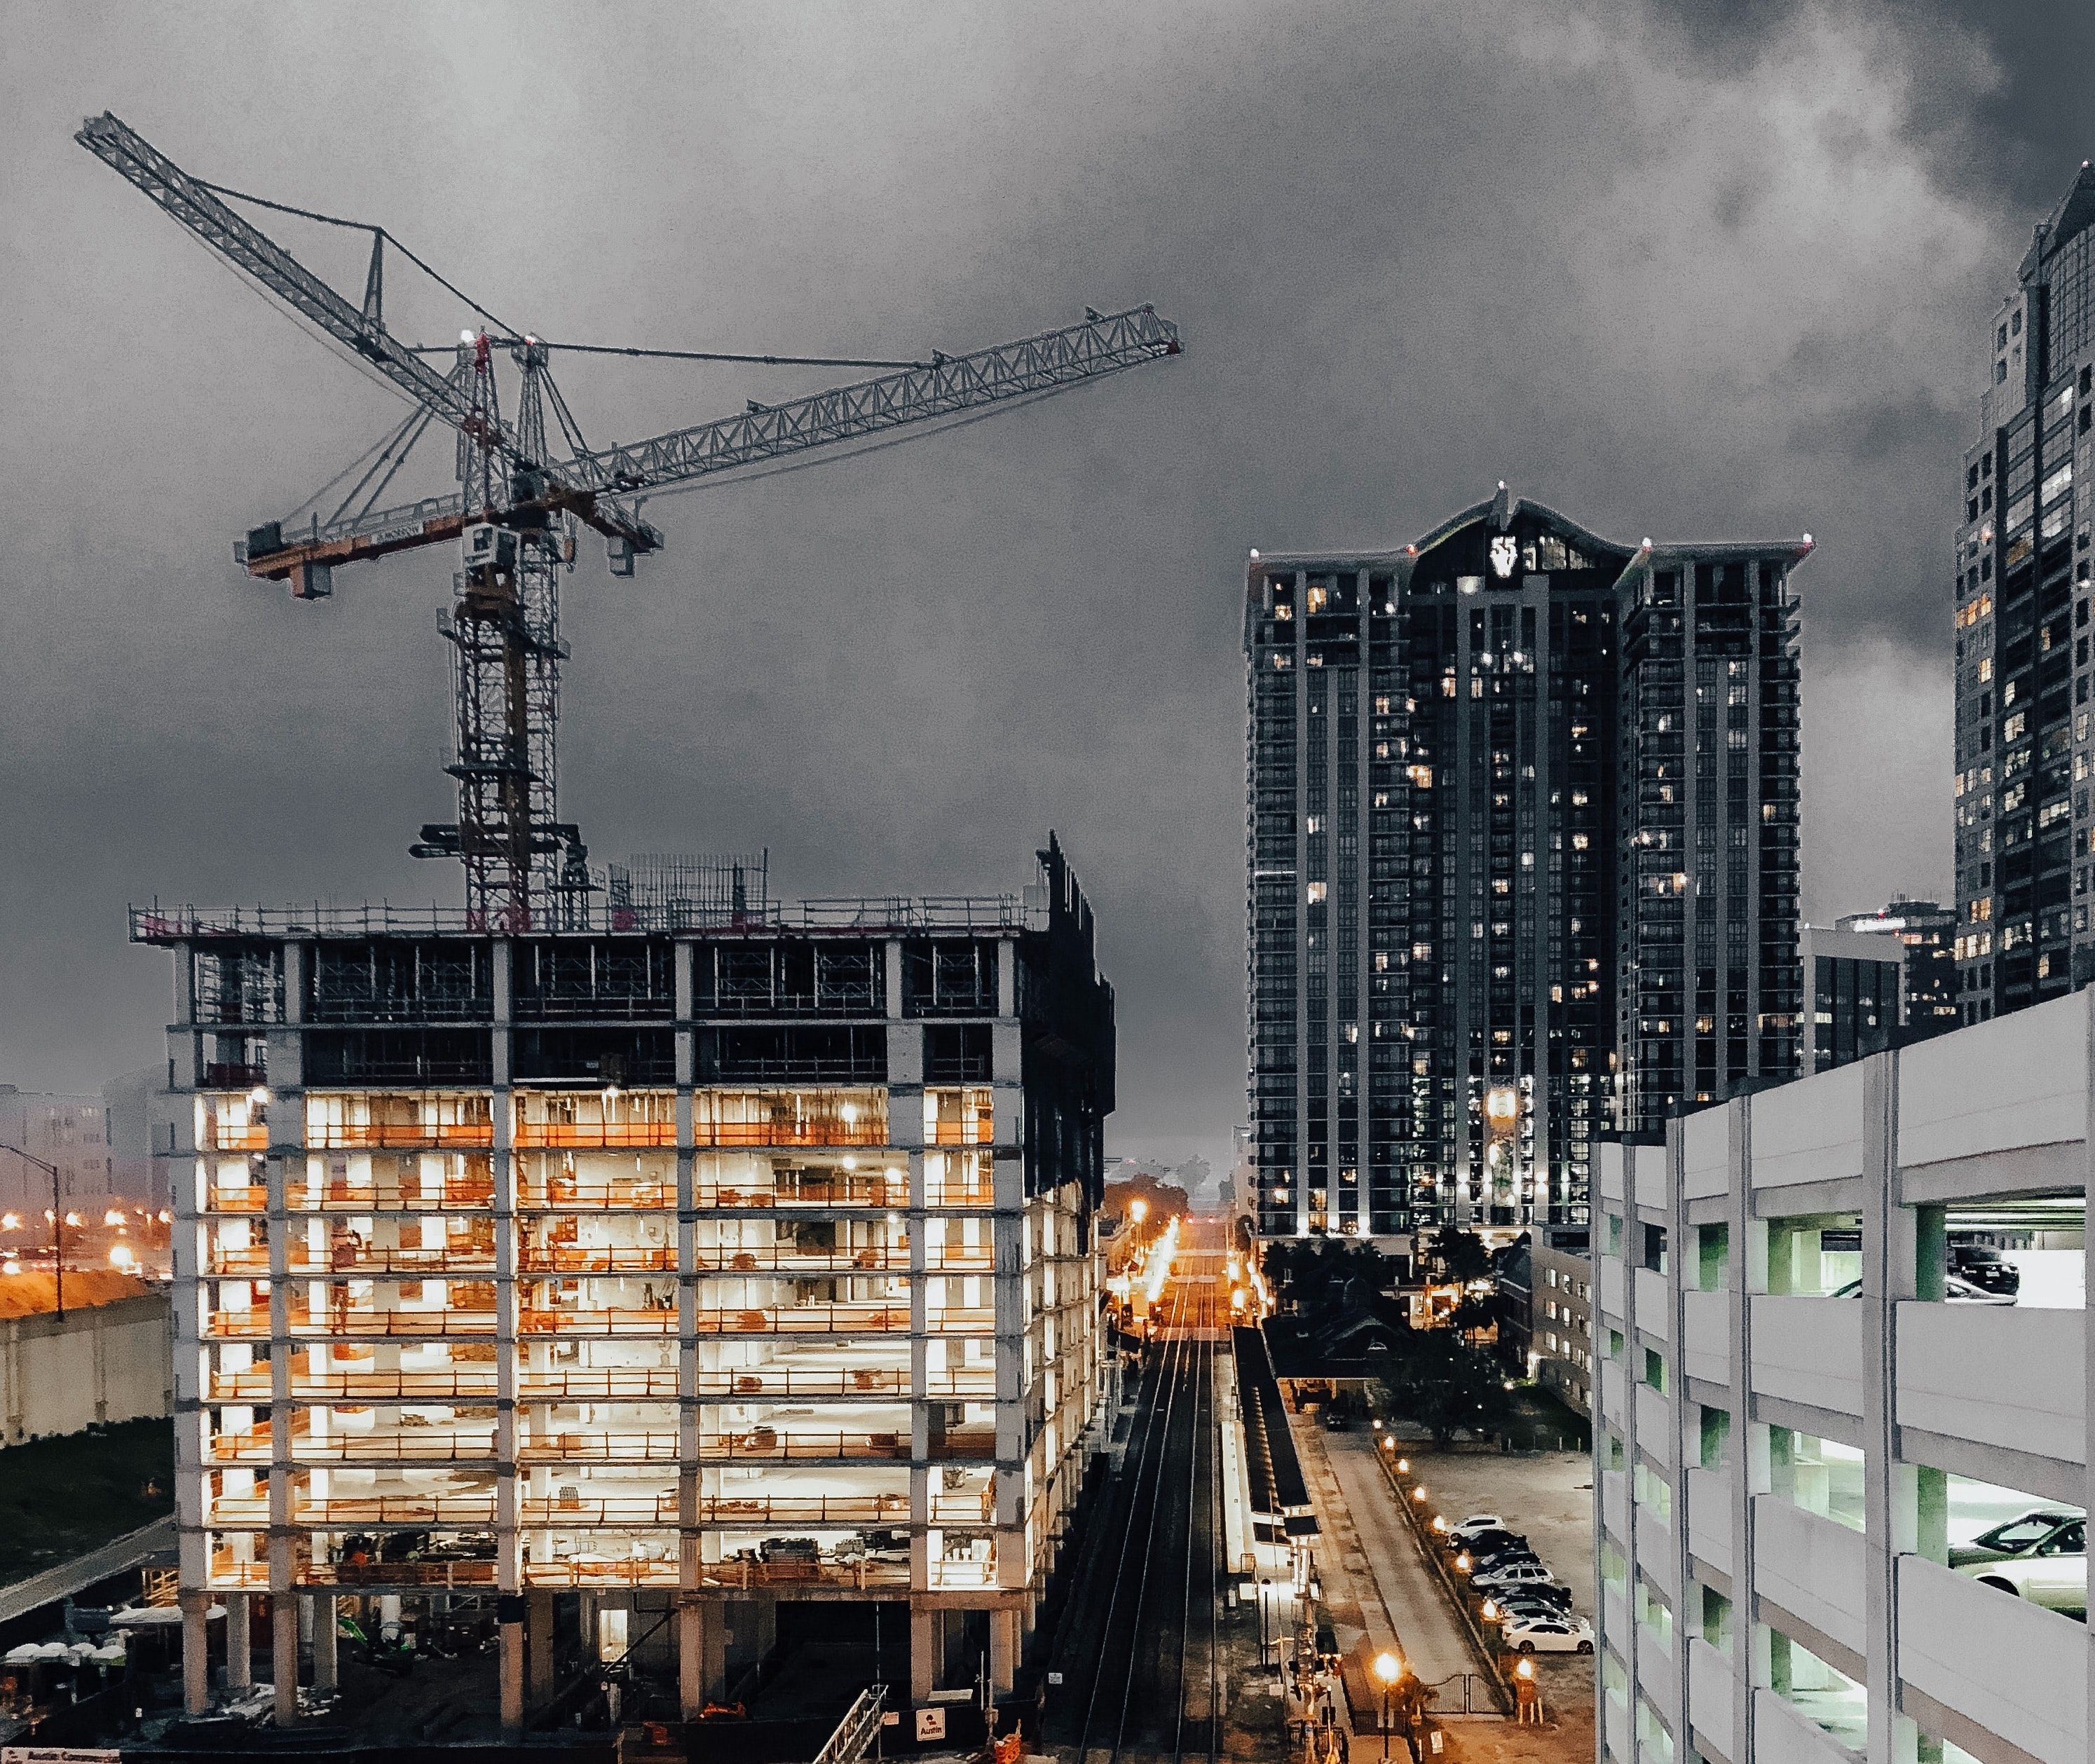
\includegraphics{img/crane.jpg} Photo by Nathan Waters on Unsplash

\end{footnotesize}}

\hypertarget{introduction}{%
\section{Introduction}\label{introduction}}

Neovim (a fork of Vim) is a text editor that has several advantages for
data science code development. One of the main attractions is that it is
open source and has a number of useful plugins to facilitate working on
R, python, and julia code. Also, its modal, keyboard-centric system
allows text and code manipulation at potentially far greater speed than
conventional, mouse-centric, systems.

In this post we describe both a minimal, yet functional setup, as well
as a more extensive setup utilizing several of the newest neovim-only
plugins, for neovim to allow IDE style code editing and REPL interaction
for the three primary data science coding tools: R, Python, and Julia.

Our presentation here is for a Macos environment. Appendix one contains
required adjustments for a ubuntu linux environment.

\hypertarget{install-the-latest-stable-version-of-neovim.}{%
\section{Install the latest stable version of
neovim.}\label{install-the-latest-stable-version-of-neovim.}}

With minimal effort we can install both the terminal and GUI versions of
neovim. The simplist approach is to use homebrew:

\begin{Shaded}
\begin{Highlighting}[]
\OperatorTok{\textgreater{}}\NormalTok{ brew }\FunctionTok{install}\NormalTok{ neovim neovim{-}qt}
\end{Highlighting}
\end{Shaded}

Set up convenience aliases in \texttt{zsh}.

\begin{Shaded}
\begin{Highlighting}[]
\OperatorTok{\textgreater{}}\NormalTok{ alias }\ExtensionTok{ng}\NormalTok{ = neovim{-}qt}
\OperatorTok{\textgreater{}}\NormalTok{ alias }\ExtensionTok{nt}\NormalTok{ = neovim}
\end{Highlighting}
\end{Shaded}

(mnemonic: the \texttt{t} in \texttt{nt} is for terminal, the \texttt{g}
in \texttt{ng} is for GUI)

\hypertarget{configure-neovim}{%
\section{Configure neovim}\label{configure-neovim}}

The standard location for \texttt{neovim} configuration files on
``unix-like'' systems is \texttt{\textasciitilde{}/.config/nvim}. The
main config file is either init.vim (VimL) or init.lua (Lua). In this
post we'll focus on lua based configuration.

Specifically, the following code block creates an \texttt{nvim}
subdirectory under \texttt{\textasciitilde{}/.config} and initialize a
configuration file \texttt{init.lua}.

Here is the file hierarchy we'll construct. In fact all the code could
be bundled into the \texttt{init.lua} file, but this approach is clearer
and cleaner.

\begin{Shaded}
\begin{Highlighting}[]
\BuiltInTok{.}
\KeywordTok{|}\ExtensionTok{{-}{-}}\NormalTok{ ginit.vim}
\KeywordTok{|}\ExtensionTok{{-}{-}}\NormalTok{ init.lua}
\KeywordTok{|}\ExtensionTok{{-}{-}}\NormalTok{ lazy{-}lock.json}
\KeywordTok{|}\ExtensionTok{{-}{-}}\NormalTok{ lua}
\KeywordTok{|}   \KeywordTok{|}\ExtensionTok{{-}{-}}\NormalTok{ basics.lua}
\KeywordTok{|}   \KeywordTok{|}\ExtensionTok{{-}{-}}\NormalTok{ leap{-}config.lua}
\KeywordTok{|}   \KeywordTok{|}\ExtensionTok{{-}{-}}\NormalTok{ nvim{-}R{-}config.lua}
\KeywordTok{|}   \KeywordTok{|}\ExtensionTok{{-}{-}}\NormalTok{ nvim{-}cmp{-}config.lua}
\KeywordTok{|}   \KeywordTok{|}\ExtensionTok{{-}{-}}\NormalTok{ nvim{-}telescope{-}config.lua}
\KeywordTok{|}   \KeywordTok{|}\ExtensionTok{{-}{-}}\NormalTok{ nvim{-}tree{-}config.lua}
\KeywordTok{|}   \KeywordTok{\textasciigrave{}}\ExtensionTok{{-}{-}}\NormalTok{ treesitter{-}config.lua}
\KeywordTok{|}\ExtensionTok{{-}{-}}\NormalTok{ my\_snippets}
\KeywordTok{|}   \KeywordTok{|}\ExtensionTok{{-}{-}}\NormalTok{ all.snippets}
\KeywordTok{|}   \KeywordTok{|}\ExtensionTok{{-}{-}}\NormalTok{ giles.tex.snipppets}
\KeywordTok{|}   \KeywordTok{|}\ExtensionTok{{-}{-}}\NormalTok{ mail.snippets}
\KeywordTok{|}   \KeywordTok{|}\ExtensionTok{{-}{-}}\NormalTok{ r.snippets}
\KeywordTok{|}   \KeywordTok{|}\ExtensionTok{{-}{-}}\NormalTok{ rmd.snippets}
\KeywordTok{|}   \KeywordTok{|}\ExtensionTok{{-}{-}}\NormalTok{ snippets.snippets}
\KeywordTok{|}   \KeywordTok{|}\ExtensionTok{{-}{-}}\NormalTok{ tex.snippets}
\KeywordTok{|}   \KeywordTok{|}\ExtensionTok{{-}{-}}\NormalTok{ text.snippets}
\KeywordTok{|}   \KeywordTok{\textasciigrave{}}\AttributeTok{{-}{-}}\NormalTok{ txt.snippets}
\KeywordTok{|}\ExtensionTok{{-}{-}}\NormalTok{ spell}
\KeywordTok{|}   \KeywordTok{|}\ExtensionTok{{-}{-}}\NormalTok{ en.utf{-}8.add}
\KeywordTok{|}   \KeywordTok{\textasciigrave{}}\ExtensionTok{{-}{-}}\NormalTok{ en.utf{-}8.add.spl}
\end{Highlighting}
\end{Shaded}

To install the \texttt{lazy} plugin manager

\begin{Shaded}
\begin{Highlighting}[]
\FunctionTok{git}\NormalTok{ clone https://github.com/folke/lazy.nvim.git }\DataTypeTok{\textbackslash{}}
\NormalTok{   \textasciitilde{}/.local/share/nvim/lazy/lazy.nvim}
\end{Highlighting}
\end{Shaded}

Add the following code to \texttt{init.lua} list the plugins needed to
be installed from \texttt{github} and ``feed'' them to \texttt{Lazy} for
installation.

Nvim-R, Leap, UltiSnips, and vimtex need additional configuration. The
required code is contained in bespoke files under the \texttt{lua}
directory.

\begin{Shaded}
\begin{Highlighting}[]


\ExtensionTok{vim.g.mapleader}\NormalTok{ = }\StringTok{" "}
\ExtensionTok{vim.g.maplocalleader}\NormalTok{ = }\StringTok{","}
\ExtensionTok{vim.opt.rtp:prepend}\ErrorTok{(}\StringTok{"\textasciitilde{}/.local/share/nvim/lazy/lazy.nvim"}\KeywordTok{)}
\ExtensionTok{require}\ErrorTok{(}\StringTok{\textquotesingle{}plugins\textquotesingle{}}\KeywordTok{)}

\ExtensionTok{require}\ErrorTok{(}\StringTok{\textquotesingle{}nvim{-}cmp{-}config\textquotesingle{}}\KeywordTok{)}
\ExtensionTok{require}\StringTok{\textquotesingle{}lspconfig\textquotesingle{}}\ExtensionTok{.lua\_ls.setup\{\}}
\ExtensionTok{require}\StringTok{\textquotesingle{}lspconfig\textquotesingle{}}\ExtensionTok{.r\_language\_server.setup\{\}}

\ExtensionTok{require}\ErrorTok{(}\StringTok{\textquotesingle{}basics\textquotesingle{}}\KeywordTok{)}
\ExtensionTok{require}\ErrorTok{(}\StringTok{\textquotesingle{}nvim{-}tree{-}config\textquotesingle{}}\KeywordTok{)}
\ExtensionTok{require}\ErrorTok{(}\StringTok{\textquotesingle{}nvim{-}R{-}config\textquotesingle{}}\KeywordTok{)}
\ExtensionTok{require}\ErrorTok{(}\StringTok{\textquotesingle{}nvim{-}telescope{-}config\textquotesingle{}}\KeywordTok{)}
\ExtensionTok{require}\ErrorTok{(}\StringTok{\textquotesingle{}leap\textquotesingle{}}\KeywordTok{)}\FunctionTok{.add\_default\_mappings()}
\ExtensionTok{require}\ErrorTok{(}\StringTok{\textquotesingle{}leap{-}config\textquotesingle{}}\KeywordTok{)}

\ExtensionTok{vim.api.nvim\_create\_autocmd}\ErrorTok{(}\StringTok{\textquotesingle{}LspAttach\textquotesingle{}}\ExtensionTok{,}\NormalTok{ \{}
  \ExtensionTok{desc}\NormalTok{ = }\StringTok{\textquotesingle{}LSP actions\textquotesingle{}}\NormalTok{,}
  \ExtensionTok{callback}\NormalTok{ = function}\ErrorTok{(}\KeywordTok{)}
    \BuiltInTok{local} \VariableTok{bufmap} \OperatorTok{=} \VariableTok{function(}\NormalTok{mode, lhs, rhs}\VariableTok{)}
      \BuiltInTok{local} \VariableTok{opts} \OperatorTok{=}\NormalTok{ \{buffer }\OperatorTok{=} \VariableTok{true}\NormalTok{\}}
      \ExtensionTok{vim.keymap.set}\ErrorTok{(}\ExtensionTok{mode,}\NormalTok{ lhs, rhs, opts}\KeywordTok{)}
    \ExtensionTok{end}
    \ExtensionTok{bufmap}\ErrorTok{(}\StringTok{\textquotesingle{}n\textquotesingle{}}\ExtensionTok{,} \StringTok{\textquotesingle{}K\textquotesingle{}}\NormalTok{, }\StringTok{\textquotesingle{}\textless{}cmd\textgreater{}lua vim.lsp.buf.hover()\textless{}cr\textgreater{}\textquotesingle{}}\KeywordTok{)}
    \ExtensionTok{bufmap}\ErrorTok{(}\StringTok{\textquotesingle{}n\textquotesingle{}}\ExtensionTok{,} \StringTok{\textquotesingle{}gl\textquotesingle{}}\NormalTok{, }\StringTok{\textquotesingle{}\textless{}cmd\textgreater{}lua vim.diagnostic.open\_float()\textless{}cr\textgreater{}\textquotesingle{}}\KeywordTok{)}
    \ExtensionTok{bufmap}\ErrorTok{(}\StringTok{\textquotesingle{}n\textquotesingle{}}\ExtensionTok{,} \StringTok{\textquotesingle{}[d\textquotesingle{}}\NormalTok{, }\StringTok{\textquotesingle{}\textless{}cmd\textgreater{}lua vim.diagnostic.goto\_prev()\textless{}cr\textgreater{}\textquotesingle{}}\KeywordTok{)}
    \ExtensionTok{bufmap}\ErrorTok{(}\StringTok{\textquotesingle{}n\textquotesingle{}}\ExtensionTok{,} \StringTok{\textquotesingle{}]d\textquotesingle{}}\NormalTok{, }\StringTok{\textquotesingle{}\textless{}cmd\textgreater{}lua vim.diagnostic.goto\_next()\textless{}cr\textgreater{}\textquotesingle{}}\KeywordTok{)}
  \ExtensionTok{end}
\ErrorTok{\}}\KeywordTok{)}
\end{Highlighting}
\end{Shaded}

List of plugins

\begin{Shaded}
\begin{Highlighting}[]

\ExtensionTok{require}\ErrorTok{(}\StringTok{\textquotesingle{}lazy\textquotesingle{}}\KeywordTok{)}\ExtensionTok{.setup}\ErrorTok{(}\KeywordTok{\{}
\ExtensionTok{{-}{-}}
\ExtensionTok{{-}{-}minimal}\NormalTok{ data science setup}
\ExtensionTok{{-}{-}}
\StringTok{\textquotesingle{}jalvesaq/Nvim{-}R\textquotesingle{}}\ExtensionTok{,}
\StringTok{\textquotesingle{}lervag/vimtex\textquotesingle{}}\ExtensionTok{,}
\StringTok{\textquotesingle{}SirVer/ultisnips\textquotesingle{}}\ExtensionTok{,}
\StringTok{\textquotesingle{}honza/vim{-}snippets\textquotesingle{}}\ExtensionTok{,}
\StringTok{\textquotesingle{}jmbuhr/otter.nvim\textquotesingle{}}\ExtensionTok{,}
\StringTok{\textquotesingle{}quarto{-}dev/quarto{-}nvim\textquotesingle{}}\ExtensionTok{,}
\StringTok{\textquotesingle{}jalvesaq/vimcmdline\textquotesingle{}}\ExtensionTok{,}
\ExtensionTok{{-}{-}}
\ExtensionTok{{-}{-}optional}\NormalTok{ utilities}
\ExtensionTok{{-}{-}}
\KeywordTok{\{} \StringTok{"bluz71/vim{-}moonfly{-}colors"}\ExtensionTok{,}\NormalTok{ name = }\StringTok{"moonfly"}\NormalTok{, lazy = false, priority = 1000 \},}
\StringTok{\textquotesingle{}junegunn/vim{-}peekaboo\textquotesingle{}}\ExtensionTok{,}
\StringTok{\textquotesingle{}preservim/nerdcommenter\textquotesingle{}}\ExtensionTok{,}
\StringTok{\textquotesingle{}machakann/vim{-}highlightedyank\textquotesingle{}}\ExtensionTok{,}
\StringTok{\textquotesingle{}kylechui/nvim{-}surround\textquotesingle{}}\ExtensionTok{,}
\ExtensionTok{{-}{-}}\StringTok{\textquotesingle{}junegunn/fzf\textquotesingle{}}\ExtensionTok{,}
\StringTok{\textquotesingle{}ggandor/leap.nvim\textquotesingle{}}\ExtensionTok{,}
\ExtensionTok{{-}{-}}\StringTok{\textquotesingle{}rhysd/clever{-}f.vim\textquotesingle{}}\ExtensionTok{,}
\StringTok{\textquotesingle{}junegunn/goyo.vim\textquotesingle{}}\ExtensionTok{,}
\StringTok{\textquotesingle{}junegunn/limelight.vim\textquotesingle{}}\ExtensionTok{,}
\StringTok{\textquotesingle{}junegunn/vim{-}easy{-}align\textquotesingle{}}\ExtensionTok{,}
\StringTok{\textquotesingle{}voldikss/vim{-}floaterm\textquotesingle{}}\ExtensionTok{,}
\ExtensionTok{{-}{-}}
\ExtensionTok{{-}{-}neovim}\NormalTok{ specific}
\ExtensionTok{{-}{-}}
\StringTok{\textquotesingle{}nvim{-}lua/plenary.nvim\textquotesingle{}}\ExtensionTok{,}
\StringTok{\textquotesingle{}nvim{-}tree/nvim{-}web{-}devicons\textquotesingle{}}\ExtensionTok{,}
\StringTok{\textquotesingle{}nvim{-}tree/nvim{-}tree.lua\textquotesingle{}}\ExtensionTok{,}
\StringTok{\textquotesingle{}nvim{-}telescope/telescope.nvim\textquotesingle{}}\ExtensionTok{,}
\StringTok{\textquotesingle{}nvim{-}treesitter/nvim{-}treesitter\textquotesingle{}}\ExtensionTok{,}
\StringTok{\textquotesingle{}neovim/nvim{-}lspconfig\textquotesingle{}}\ExtensionTok{,}
\StringTok{\textquotesingle{}hrsh7th/nvim{-}cmp\textquotesingle{}}\ExtensionTok{,}
\StringTok{\textquotesingle{}uga{-}rosa/cmp{-}dictionary\textquotesingle{}}\ExtensionTok{,}
\StringTok{\textquotesingle{}tamago324/cmp{-}zsh\textquotesingle{}}\ExtensionTok{,}
\ExtensionTok{{-}{-}}\StringTok{\textquotesingle{}hrsh7th/cmp{-}nvim{-}lsp{-}signature{-}help\textquotesingle{}}\ExtensionTok{,}
\StringTok{\textquotesingle{}hrsh7th/cmp{-}nvim{-}lsp\textquotesingle{}}\ExtensionTok{,}
\StringTok{\textquotesingle{}hrsh7th/cmp{-}buffer\textquotesingle{}}\ExtensionTok{,}
\StringTok{\textquotesingle{}hrsh7th/cmp{-}path\textquotesingle{}}\ExtensionTok{,}
\StringTok{\textquotesingle{}hrsh7th/cmp{-}cmdline\textquotesingle{}}\ExtensionTok{,}
\StringTok{\textquotesingle{}quangnguyen30192/cmp{-}nvim{-}ultisnips\textquotesingle{}}\ExtensionTok{,}
\StringTok{\textquotesingle{}jalvesaq/cmp{-}nvim{-}r\textquotesingle{}}\ExtensionTok{,}
\StringTok{\textquotesingle{}LuaLS/lua{-}language{-}server\textquotesingle{}}\ExtensionTok{,}
\KeywordTok{\}}\ErrorTok{)}
\end{Highlighting}
\end{Shaded}

\hypertarget{plugin-discussions}{%
\section{plugin discussions}\label{plugin-discussions}}

\hypertarget{cmp-config}{%
\section{cmp config}\label{cmp-config}}

\begin{Shaded}
\begin{Highlighting}[]

\BuiltInTok{local} \VariableTok{kind\_icons} \OperatorTok{=}\NormalTok{ \{}
  \ExtensionTok{Function}\NormalTok{ = }\StringTok{"f"}\NormalTok{,}
  \ExtensionTok{Snippet}\NormalTok{ = }\StringTok{"s"}\NormalTok{,}
  \ExtensionTok{Text}\NormalTok{ = }\StringTok{"t"}\NormalTok{,}
\ErrorTok{\}}

\BuiltInTok{local} \VariableTok{cmp\_ultisnips\_mappings} \OperatorTok{=} \VariableTok{require(}\StringTok{"cmp\_nvim\_ultisnips.mappings"}\VariableTok{)}
\BuiltInTok{local} \VariableTok{cmp} \OperatorTok{=} \VariableTok{require}\StringTok{\textquotesingle{}cmp\textquotesingle{}}
\ExtensionTok{{-}{-}local}\NormalTok{ lspkind = require}\ErrorTok{(}\StringTok{\textquotesingle{}lspkind\textquotesingle{}}\KeywordTok{)}

\BuiltInTok{local} \VariableTok{mappings} \OperatorTok{=}\NormalTok{ \{}
  \ExtensionTok{[}\StringTok{"\textless{}Tab\textgreater{}"}\ExtensionTok{]}\NormalTok{ = cmp.mapping}\ErrorTok{(}
    \KeywordTok{function(}\ExtensionTok{fallback}\KeywordTok{)}
      \ExtensionTok{cmp\_ultisnips\_mappings.compose}\NormalTok{ \{ }\StringTok{"select\_next\_item"}\NormalTok{ \}}\ErrorTok{(}\ExtensionTok{fallback}\KeywordTok{)}
    \ExtensionTok{end,}
    \KeywordTok{\{} \StringTok{"i"}\ExtensionTok{,} \StringTok{"s"}\NormalTok{, }\AttributeTok{{-}{-}[[} \StringTok{"c"} \ErrorTok{(}\ExtensionTok{to}\NormalTok{ enable the mapping in command mode}\KeywordTok{)} \ExtensionTok{]]}\NormalTok{ \}}
  \ErrorTok{)}\ExtensionTok{,}
  \ExtensionTok{[}\StringTok{"\textless{}S{-}Tab\textgreater{}"}\ExtensionTok{]}\NormalTok{ = cmp.mapping}\ErrorTok{(}
    \KeywordTok{function(}\ExtensionTok{fallback}\KeywordTok{)}
      \ExtensionTok{cmp\_ultisnips\_mappings.compose}\NormalTok{ \{ }\StringTok{"select\_prev\_item"}\NormalTok{ \}}\ErrorTok{(}\ExtensionTok{fallback}\KeywordTok{)}
    \ExtensionTok{end,}
    \KeywordTok{\{} \StringTok{"i"}\ExtensionTok{,} \StringTok{"s"}\NormalTok{, }\AttributeTok{{-}{-}[[} \StringTok{"c"} \ErrorTok{(}\ExtensionTok{to}\NormalTok{ enable the mapping in command mode}\KeywordTok{)} \ExtensionTok{]]}\NormalTok{ \}}
  \ErrorTok{)}\ExtensionTok{,}
\KeywordTok{\}}

\ExtensionTok{cmp.setup}\ErrorTok{(}\KeywordTok{\{}
\ExtensionTok{window}\NormalTok{ = \{}
    \ExtensionTok{completion}\NormalTok{ = cmp.config.window.bordered}\ErrorTok{(}\KeywordTok{)}\ExtensionTok{,}
    \ExtensionTok{documentation}\NormalTok{ = cmp.config.window.bordered}\ErrorTok{(}\KeywordTok{)}\ExtensionTok{,}
  \ExtensionTok{\},}
\ExtensionTok{formatting}\NormalTok{ = \{}
\ExtensionTok{format}\NormalTok{ = function}\ErrorTok{(}\ExtensionTok{entry,}\NormalTok{ vim\_item}\KeywordTok{)}
      \ExtensionTok{vim\_item.kind}\NormalTok{ = string.format}\ErrorTok{(}\StringTok{"\%s \%s"}\ExtensionTok{,}\NormalTok{ kind\_icons[vim\_item.kind], vim\_item.kind}\KeywordTok{)} \ExtensionTok{{-}{-}Concatonate}\NormalTok{ the icons with name of the item{-}kind}
      \ExtensionTok{vim\_item.menu}\NormalTok{ = }\ErrorTok{(}\KeywordTok{\{}
        \ExtensionTok{spell}\NormalTok{ = }\StringTok{"[Spellings]"}\NormalTok{,}
        \ExtensionTok{ultisnips}\NormalTok{ = }\StringTok{"[Snip]"}\NormalTok{,}
        \ExtensionTok{cmp\_nvim\_r}\NormalTok{ = }\StringTok{"[R]"}\NormalTok{,}
      \KeywordTok{\})}\ExtensionTok{[entry.source.name]}
      \ControlFlowTok{return} \ExtensionTok{vim\_item}
    \ExtensionTok{end,}
    \ExtensionTok{\},}
  \ExtensionTok{snippet}\NormalTok{ = \{}
    \FunctionTok{expand}\NormalTok{ = function}\ErrorTok{(}\ExtensionTok{args}\KeywordTok{)}
      \ExtensionTok{vim.fn[}\StringTok{"UltiSnips\#Anon"}\ExtensionTok{]}\ErrorTok{(}\ExtensionTok{args.body}\KeywordTok{)} 
    \ExtensionTok{end,}
  \ExtensionTok{\},}

\ExtensionTok{sources}\NormalTok{ = cmp.config.sources}\ErrorTok{(}\KeywordTok{\{}
    \KeywordTok{\{} \ExtensionTok{name}\NormalTok{ = }\StringTok{"nvim\_lsp"}\NormalTok{ \},}
    \KeywordTok{\{} \ExtensionTok{name}\NormalTok{ = }\StringTok{\textquotesingle{}cmp\_nvim\_r\textquotesingle{}}\NormalTok{ \},}
    \KeywordTok{\{} \ExtensionTok{name}\NormalTok{ = }\StringTok{\textquotesingle{}nvim\_lua\textquotesingle{}}\NormalTok{ \},}
    \KeywordTok{\{} \ExtensionTok{name}\NormalTok{ = }\StringTok{"ultisnips"}\NormalTok{ \},}
    \KeywordTok{\{} \ExtensionTok{name}\NormalTok{ = }\StringTok{"dictionary"}\NormalTok{, keyword\_length=4, \},}
    \KeywordTok{\{} \ExtensionTok{name}\NormalTok{ = }\StringTok{"buffer"}\NormalTok{, option = \{ get\_bufnrs = function}\ErrorTok{(}\KeywordTok{)}
      \ControlFlowTok{return} \FunctionTok{vim.api.nvim\_list\_bufs()}
    \ExtensionTok{end}
    \ExtensionTok{\}\},}
    \KeywordTok{\{} \ExtensionTok{name}\NormalTok{ = }\StringTok{"path"}\NormalTok{ \},}
    \KeywordTok{\{} \ExtensionTok{name}\NormalTok{ = }\StringTok{"calc"}\NormalTok{ \}}
  \KeywordTok{\}}\ErrorTok{)}\ExtensionTok{,}
  \ExtensionTok{mapping}\NormalTok{ = mappings,}
\KeywordTok{\}}\ErrorTok{)}

  \ExtensionTok{require}\ErrorTok{(}\StringTok{\textquotesingle{}lspconfig\textquotesingle{}}\KeywordTok{)}\ExtensionTok{[}\StringTok{\textquotesingle{}r\_language\_server\textquotesingle{}}\ExtensionTok{].setup}\NormalTok{ \{}
    \ExtensionTok{capabilities}\NormalTok{ = capabilities}
  \KeywordTok{\}}

\ExtensionTok{require}\StringTok{\textquotesingle{}cmp\_nvim\_r\textquotesingle{}}\ExtensionTok{.setup}\ErrorTok{(}\KeywordTok{\{}
  \ExtensionTok{filetypes}\NormalTok{ = \{}\StringTok{\textquotesingle{}r\textquotesingle{}}\NormalTok{, }\StringTok{\textquotesingle{}rmd\textquotesingle{}}\NormalTok{, }\StringTok{\textquotesingle{}quarto\textquotesingle{}}\NormalTok{\},}
  \ExtensionTok{doc\_width}\NormalTok{ = 58}
  \KeywordTok{\})}
\end{Highlighting}
\end{Shaded}

\hypertarget{basics}{%
\section{basics}\label{basics}}

\begin{Shaded}
\begin{Highlighting}[]


\BuiltInTok{local} \VariableTok{map} \OperatorTok{=} \VariableTok{vim}\NormalTok{.keymap.set}
\BuiltInTok{local} \VariableTok{opts} \OperatorTok{=}\NormalTok{ \{noremap }\OperatorTok{=} \VariableTok{true}\NormalTok{\}}
\ExtensionTok{vim.cmd}\ErrorTok{(}\KeywordTok{[[}
\StringTok{"    copy clipboard to register x for safe keeping}
\StringTok{nnoremap \textless{}leader\textgreater{}x :let @x=@*}
\StringTok{"}\NormalTok{    paste registers }\ErrorTok{into} \ExtensionTok{terminal}
\ExtensionTok{tnoremap} \OperatorTok{\textless{}}\NormalTok{expr}\OperatorTok{\textgreater{}} \OperatorTok{\textless{}}\NormalTok{C{-}R}\OperatorTok{\textgreater{}} \StringTok{\textquotesingle{}\textless{}C{-}\textbackslash{}\textgreater{}\textless{}C{-}N\textgreater{}"\textquotesingle{}}\NormalTok{.nr2char}\ErrorTok{(}\FunctionTok{getchar()}\KeywordTok{)}\ExtensionTok{.}\StringTok{\textquotesingle{}pi\textquotesingle{}}
\BuiltInTok{set}\NormalTok{ background=dark}
\StringTok{"colorscheme evening}
\StringTok{colorscheme moonfly}
\StringTok{let }\VariableTok{$FZF\_DEFAULT\_COMMAND}\StringTok{ = \textquotesingle{}rg {-}{-}files {-}{-}hidden\textquotesingle{}}
\StringTok{set completeopt=menu,menuone,noinsert,noselect}
\StringTok{set number relativenumber}
\StringTok{set textwidth=80}
\StringTok{set cursorline}
\StringTok{set clipboard=unnamed}
\StringTok{set iskeyword{-}=\_ }
\StringTok{set hlsearch   }
\StringTok{set splitright}
\StringTok{set hidden   }
\StringTok{set incsearch    }
\StringTok{set noswapfile}
\StringTok{set showmatch}
\StringTok{set ignorecase}
\StringTok{set smartcase}
\StringTok{set gdefault}
\StringTok{filetype plugin on}
\StringTok{set encoding=utf{-}8}
\StringTok{set nobackup}
\StringTok{set nowritebackup}
\StringTok{set updatetime=300}
\StringTok{set signcolumn=yes}
\StringTok{set colorcolumn=80}
\StringTok{autocmd! User GoyoEnter Limelight}
\StringTok{autocmd! User GoyoLeave Limelight!}

\StringTok{set dictionary+=/usr/share/dict/words}
\StringTok{set thesaurus+=/Users/zenn/mthesaur.txt}

\StringTok{let g:UltiSnipsSnippetDirectories=["}\ExtensionTok{UltiSnips}\StringTok{", "}\ExtensionTok{my\_snippets}\StringTok{"]}
\StringTok{let g:UltiSnipsEditSplit="}\ExtensionTok{vertical}\StringTok{"}
\StringTok{let g:UltiSnipsUsePythonVersion = 3}

\StringTok{autocmd FileType julia,python nnoremap \textless{}buffer\textgreater{} \textless{}C{-}CR\textgreater{}  :call VimCmdLineStartApp()\textless{}CR\textgreater{}}
\StringTok{autocmd FileType julia,python nnoremap \textless{}buffer\textgreater{} \textless{}CR\textgreater{}  :call VimCmdLineSendLine()\textless{}CR\textgreater{}}
\StringTok{]])}
\StringTok{map(\textquotesingle{}n\textquotesingle{}, \textquotesingle{}:\textquotesingle{}, \textquotesingle{};\textquotesingle{}, opts)}
\StringTok{map(\textquotesingle{}n\textquotesingle{}, \textquotesingle{};\textquotesingle{}, \textquotesingle{}:\textquotesingle{}, opts)}
\StringTok{map(\textquotesingle{}n\textquotesingle{}, \textquotesingle{}\textless{}leader\textgreater{}u\textquotesingle{},\textquotesingle{}:UltiSnipsEdit\textless{}cr\textgreater{}\textquotesingle{}, opts)}
\StringTok{map(\textquotesingle{}n\textquotesingle{}, \textquotesingle{}\textless{}Space\textgreater{}\textless{}Space\textgreater{}\textquotesingle{},\textquotesingle{}\textless{}C{-}d\textgreater{}\textquotesingle{}, opts)}
\StringTok{map(\textquotesingle{}n\textquotesingle{}, \textquotesingle{}{-}\textquotesingle{},\textquotesingle{}$\textquotesingle{}, opts)}
\StringTok{map(\textquotesingle{}n\textquotesingle{}, \textquotesingle{}\textless{}leader\textgreater{}w\textquotesingle{},\textquotesingle{}vipgq\textquotesingle{}, opts)}
\StringTok{map(\textquotesingle{}n\textquotesingle{}, \textquotesingle{}\textless{}leader\textgreater{}v\textquotesingle{},\textquotesingle{}:edit \textasciitilde{}/.config/nvim/init.lua\textless{}cr\textgreater{}\textquotesingle{}, opts)}
\StringTok{map(\textquotesingle{}n\textquotesingle{}, \textquotesingle{}\textless{}leader\textgreater{}n\textquotesingle{},\textquotesingle{}:edit \textasciitilde{}/.config/nvim/lua/basics.lua\textless{}cr\textgreater{}\textquotesingle{}, opts)}
\StringTok{map(\textquotesingle{}n\textquotesingle{}, \textquotesingle{}\textless{}leader\textgreater{}a\textquotesingle{},\textquotesingle{}ggVG\textquotesingle{}, opts)}
\StringTok{map(\textquotesingle{}n\textquotesingle{}, \textquotesingle{}\textless{}leader\textgreater{}t\textquotesingle{},\textquotesingle{}:tab split\textless{}cr\textgreater{}\textquotesingle{}, opts)}
\StringTok{map(\textquotesingle{}n\textquotesingle{}, \textquotesingle{}\textless{}leader\textgreater{}y\textquotesingle{},\textquotesingle{}:vert sb3\textless{}cr\textgreater{}\textquotesingle{}, opts)}
\StringTok{map(\textquotesingle{}n\textquotesingle{}, \textquotesingle{}\textless{}leader\textgreater{}0\textquotesingle{},\textquotesingle{}:ls!\textless{}CR\textgreater{}:b\textless{}Space\textgreater{}\textquotesingle{}, opts)}
\StringTok{map(\textquotesingle{}n\textquotesingle{}, \textquotesingle{}\textless{}localleader\textgreater{}\textless{}localleader\textgreater{}\textquotesingle{},\textquotesingle{}\textless{}C{-}w\textgreater{}w\textquotesingle{}, opts)}
\StringTok{map(\textquotesingle{}n\textquotesingle{}, \textquotesingle{}\textless{}leader\textgreater{}1\textquotesingle{},\textquotesingle{}\textless{}C{-}w\textgreater{}:b1\textless{}cr\textgreater{}\textquotesingle{}, opts)}
\StringTok{map(\textquotesingle{}n\textquotesingle{}, \textquotesingle{}\textless{}leader\textgreater{}2\textquotesingle{},\textquotesingle{}\textless{}C{-}w\textgreater{}:b2\textless{}cr\textgreater{}\textquotesingle{}, opts)}
\StringTok{map(\textquotesingle{}n\textquotesingle{}, \textquotesingle{}\textless{}leader\textgreater{}3\textquotesingle{},\textquotesingle{}\textless{}C{-}w\textgreater{}:b3\textless{}cr\textgreater{}\textquotesingle{}, opts)}
\StringTok{map(\textquotesingle{}n\textquotesingle{}, \textquotesingle{}\textless{}leader\textgreater{}4\textquotesingle{},\textquotesingle{}\textless{}C{-}w\textgreater{}:b4\textless{}cr\textgreater{}\textquotesingle{}, opts)}
\StringTok{map(\textquotesingle{}n\textquotesingle{}, \textquotesingle{}\textless{}leader\textgreater{}5\textquotesingle{},\textquotesingle{}\textless{}C{-}w\textgreater{}:b5\textless{}cr\textgreater{}\textquotesingle{}, opts)}
\StringTok{map(\textquotesingle{}n\textquotesingle{}, \textquotesingle{}\textless{}leader\textgreater{}6\textquotesingle{},\textquotesingle{}\textless{}C{-}w\textgreater{}:b6\textless{}cr\textgreater{}\textquotesingle{}, opts)}
\StringTok{map(\textquotesingle{}n\textquotesingle{}, \textquotesingle{}\textless{}leader\textgreater{}7\textquotesingle{},\textquotesingle{}\textless{}C{-}w\textgreater{}:b7\textless{}cr\textgreater{}\textquotesingle{}, opts)}
\StringTok{map(\textquotesingle{}n\textquotesingle{}, \textquotesingle{}\textless{}leader\textgreater{}8\textquotesingle{},\textquotesingle{}\textless{}C{-}w\textgreater{}:b8\textless{}cr\textgreater{}\textquotesingle{}, opts)}
\StringTok{map(\textquotesingle{}n\textquotesingle{}, \textquotesingle{}\textless{}leader\textgreater{}9\textquotesingle{},\textquotesingle{}\textless{}C{-}w\textgreater{}:b9\textless{}cr\textgreater{}\textquotesingle{}, opts)}
\StringTok{map(\textquotesingle{}t\textquotesingle{},  \textquotesingle{}ZZ\textquotesingle{}, "}\ExtensionTok{q}\ErrorTok{(}\StringTok{\textquotesingle{}yes\textquotesingle{}}\KeywordTok{)}\OperatorTok{\textless{}}\NormalTok{CR}\OperatorTok{\textgreater{}}\StringTok{", opts)}
\StringTok{map(\textquotesingle{}t\textquotesingle{},  \textquotesingle{}ZQ\textquotesingle{}, "}\NormalTok{q}\KeywordTok{(}\StringTok{\textquotesingle{}no\textquotesingle{}}\KeywordTok{)}\OperatorTok{\textless{}}\NormalTok{CR}\OperatorTok{\textgreater{}}\StringTok{", opts)}
\StringTok{map(\textquotesingle{}v\textquotesingle{},  \textquotesingle{}{-}\textquotesingle{}, \textquotesingle{}$\textquotesingle{}, opts)}
\StringTok{map(\textquotesingle{}t\textquotesingle{},  \textquotesingle{}\textless{}leader\textgreater{}0\textquotesingle{},\textquotesingle{}\textless{}C{-}}\DataTypeTok{\textbackslash{}\textbackslash{}}\StringTok{\textgreater{}\textless{}C{-}n\textgreater{}\textless{}C{-}w\textgreater{}:ls!\textless{}cr\textgreater{}:b\textless{}Space\textgreater{}\textquotesingle{}, opts)}
\StringTok{map(\textquotesingle{}t\textquotesingle{},  \textquotesingle{}\textless{}Escape\textgreater{}\textquotesingle{},\textquotesingle{}\textless{}C{-}}\DataTypeTok{\textbackslash{}\textbackslash{}}\StringTok{\textgreater{}\textless{}C{-}n\textgreater{}\textquotesingle{}, opts)}
\StringTok{map(\textquotesingle{}t\textquotesingle{},  \textquotesingle{}\textless{}localeader\textgreater{}\textless{}localleader\textgreater{}\textquotesingle{},\textquotesingle{}\textless{}C{-}}\DataTypeTok{\textbackslash{}\textbackslash{}}\StringTok{\textgreater{}\textless{}C{-}n\textgreater{}\textless{}C{-}w\textgreater{}w\textquotesingle{}, opts)}
\StringTok{map(\textquotesingle{}i\textquotesingle{},  \textquotesingle{}\textless{}Esc\textgreater{}\textquotesingle{}, \textquotesingle{}\textless{}Esc\textgreater{}}\KeywordTok{\textasciigrave{}}\ExtensionTok{\^{}}\StringTok{\textquotesingle{}, opts)}


\StringTok{vim.api.nvim\_create\_autocmd(}
\StringTok{    \{ "BufRead", "BufNewFile" \},}
\StringTok{    \{ pattern = \{ "*.txt", "*.md"\}, command = "setlocal spell" \}}
\StringTok{)}





\end{Highlighting}
\end{Shaded}

\hypertarget{set-up-r}{%
\section{Set up R}\label{set-up-r}}

\begin{Shaded}
\begin{Highlighting}[]

\ExtensionTok{vim.cmd}\ErrorTok{(}\KeywordTok{[[}
\NormalTok{let R\_auto\_start = }\ErrorTok{2}
\BuiltInTok{let} \VariableTok{R\_hl\_term} \OperatorTok{=} \DecValTok{0}
\BuiltInTok{let} \VariableTok{R\_clear\_line} \OperatorTok{=} \DecValTok{1}
\BuiltInTok{let} \VariableTok{R\_pdfviewer} \OperatorTok{=} \StringTok{"zathura"} 
\BuiltInTok{let} \VariableTok{R\_assign} \OperatorTok{=} \DecValTok{2}
\BuiltInTok{let} \VariableTok{R\_latexcmd} \OperatorTok{=} \OperatorTok{[}\StringTok{\textquotesingle{}xelatex\textquotesingle{}}\OperatorTok{]}
\ExtensionTok{augroup}\NormalTok{ rmarkdown}
\ExtensionTok{autocmd!}
\ExtensionTok{autocmd}\NormalTok{ FileType rmd,r nnoremap }\OperatorTok{\textless{}}\NormalTok{buffer}\OperatorTok{\textgreater{}} \OperatorTok{\textless{}}\NormalTok{CR}\OperatorTok{\textgreater{}}\NormalTok{  :call SendLineToR}\ErrorTok{(}\StringTok{"down"}\KeywordTok{)}\OperatorTok{\textless{}}\NormalTok{CR}\OperatorTok{\textgreater{}}
\ExtensionTok{autocmd}\NormalTok{ FileType rmd,r nnoremap }\OperatorTok{\textless{}}\NormalTok{buffer}\OperatorTok{\textgreater{}} \OperatorTok{\textless{}}\NormalTok{space}\OperatorTok{\textgreater{}}\StringTok{\textquotesingle{} :call RMakeRmd("default")\textless{}cr\textgreater{}}
\StringTok{autocmd FileType rmd,r noremap \textless{}space\textgreater{}i :call RAction("dim")\textless{}cr\textgreater{}}
\StringTok{autocmd FileType rmd,r noremap \textless{}space\textgreater{}h :call RAction("head")\textless{}cr\textgreater{}}
\StringTok{autocmd FileType rmd,r noremap \textless{}space\textgreater{}p :call RAction("print")\textless{}cr\textgreater{}}
\StringTok{autocmd FileType rmd,r noremap \textless{}space\textgreater{}q :call RAction("length")\textless{}cr\textgreater{}}
\StringTok{autocmd FileType rmd,r noremap \textless{}space\textgreater{}n :call RAction("nvim.names")\textless{}cr\textgreater{}}
\StringTok{autocmd FileType rmd,r vmap \textless{}buffer\textgreater{} \textless{}CR\textgreater{} \textless{}localleader\textgreater{}sd}
\StringTok{autocmd FileType rmd,r nmap \textless{}buffer\textgreater{} \textless{}space\textgreater{}j \textless{}localleader\textgreater{}gn}
\StringTok{autocmd FileType rmd,r nmap \textless{}buffer\textgreater{} \textless{}space\textgreater{}k \textless{}localleader\textgreater{}gN}
\StringTok{autocmd FileType rmd,r nmap \textless{}buffer\textgreater{} \textless{}space\textgreater{}l \textless{}localleader\textgreater{}cd}
\StringTok{augroup END}
\StringTok{]])}
\end{Highlighting}
\end{Shaded}

\hypertarget{appendix-ubuntu-tweaks}{%
\section{Appendix Ubuntu tweaks}\label{appendix-ubuntu-tweaks}}



\end{document}
